%---------------------------------------------------------------------
%   documentclass
%---------------------------------------------------------------------
\documentclass[a4paper]{article}

%---------------------------------------------------------------------
%   packages
%---------------------------------------------------------------------

\newif\ifeng
\engtrue

\ifeng
	\usepackage[english]{babel}
\else
	\usepackage[slovak]{babel}
\fi

\usepackage{mathtools}
\usepackage[enc=cp1250]{hrlatex}
\usepackage[T1]{fontenc} %pekne makcene
\usepackage{lmodern} %spolu s T1 smooth font!
\usepackage{hyperref} %odkazy
\usepackage{amsmath}
\usepackage{amsthm}
\usepackage{cite} %bibtex
\usepackage{enumitem}
\usepackage{titlesec} %section titles font size change
\usepackage{color} %for \definecolor
\usepackage{colortbl} %for \rowcolor command
\usepackage{eucal} %for nice letters like \mathcal{A}
\usepackage[tikz]{bclogo}
\usepackage{tikz}
\usepackage{scalefnt}
\usepackage{booktabs}% http://ctan.org/pkg/booktabs
\usepackage{multirow}% http://ctan.org/pkg/multirow
\usepackage{pifont} %for ticks (check symbols)
\usepackage{listings}
\usepackage{floatflt} %to have tables and text beside
\usepackage{courier}
\usepackage{subcaption}
\usepackage{bm}

%---------------------------------------------------------------------
%   margins
%---------------------------------------------------------------------
\oddsidemargin 0.0in
\evensidemargin 0.0in
\textwidth 6.1in
\textheight 23.94cm
\topmargin -0.35in

%---------------------------------------------------------------------
%   various settings
%---------------------------------------------------------------------

\setlist{nolistsep} %so that lists have normal spacing

\titleformat{\section}{\LARGE\bfseries}{\thesection}{1em}{} %section titles
\titleformat{\subsection}{\Large\bfseries}{\thesubsection}{1em}{} %subsection titles

\definecolor{tablehead}{RGB}{238,233,233} %nice smooth grey

\setlength{\parindent}{0pt} %we don't need no indentation

\graphicspath{{./pics/}} %picture dir

\definecolor{lstcolor}{RGB}{238,233,233}

\lstset{ %
    language=Octave,                % choose the language of the code
    basicstyle=\footnotesize\ttfamily,       % the size of the fonts that are used for the code
    numbers=left,                   % where to put the line-numbers
    numberstyle=\footnotesize,      % the size of the fonts that are used for the line-numbers
    stepnumber=1,                   % the step between two line-numbers. If it's 1 each line will be numbered
    numbersep=5pt,                  % how far the line-numbers are from the code
    backgroundcolor=\color{lstcolor},   % choose the background color. You must add \usepackage{color}
    showspaces=false,               % show spaces adding particular underscores
    showstringspaces=false,         % underline spaces within strings
    showtabs=false,                 % show tabs within strings adding particular underscores
    frame=single,	                % adds a frame around the code
    tabsize=2,	                    % sets default tabsize to 2 spaces
    captionpos=b,                   % sets the caption-position to bottom
    breaklines=true,                % sets automatic line breaking
    breakatwhitespace=false,        % sets if automatic breaks should only happen at whitespace
    title=\lstname,                 % show the filename of files included with \lstinputlisting; also try caption instead of title
    escapeinside={\%*}{*)},          % if you want to add a comment within your code
%    morekeywords={*,...}            % if you want to add more keywords to the set
	deletekeywords={all, null, length, path, for, line, load, set, help, hold, case, size, find}
}

%---------------------------------------------------------------------
%   environments
%---------------------------------------------------------------------
\renewenvironment{abstract}[1]
{
	\Large
	\begin{center}
		\textbf{#1}
	\end{center}
	
	\normalsize
	
	\addtolength{\leftskip}{1in}
	\addtolength{\rightskip}{1in}
	\setlength{\parindent}{0in}
}
{
}

\newenvironment{itemizesp}
{
    \begin{itemize}
}
{
    \end{itemize}
}

\newcommand{\deftoken}{\boldmath{$\mathcal{DEFINITION}$}}
\newcommand{\restoken}{\boldmath{$\mathcal{RESULT}$}}
\newcommand{\dotoken}{\boldmath{$\mathcal{DO METHOD}$}}
\newcommand{\textbff}[1]{{\large \textbf{#1}}}
\newcommand{\tick}{\ding{52}}

\newtheorem{definition}{Definition}
\newtheorem{lemma}{Lemma}
\newtheorem{observation}{Observation}

%---------------------------------------------------------------------
%   magic code
%---------------------------------------------------------------------
% Here it is: the code that adjusts justification and spacing around caption.
\makeatletter
% http://www.texnik.de/floats/caption.phtml
% This does spacing around caption.
\setlength{\abovecaptionskip}{6pt}   % 0.5cm as an example
\setlength{\belowcaptionskip}{6pt}   % 0.5cm as an example
% This does justification (left) of caption.
\long\def\@makecaption#1#2{%
  \vskip\abovecaptionskip
  \sbox\@tempboxa{#1: #2}%
  \ifdim \wd\@tempboxa >\hsize
    #1: #2\par
  \else
    \global \@minipagefalse
    \hb@xt@\hsize{\box\@tempboxa\hfil}%
  \fi
  \vskip\belowcaptionskip}
\makeatother

%---------------------------------------------------------------------
%   document
%---------------------------------------------------------------------
\begin{document}
    \thispagestyle{empty}
    %---------------------------------------------------------------------
    %   topmatter
    %---------------------------------------------------------------------
   
    \ifeng
    
    \title{\textbf{Pizzas by Fero}\\
    \textit{version 2.1}}
    \author{Franti�ek Hajnovi� \\
    \texttt{ferohajnovic@gmail.com}}
    \date{\today}

	\else
	
	\title{\textbf{Ferove pizze}\\
    \textit{verzia 2.0}}
    \author{Franti�ek Hajnovi� \\
    \texttt{ferohajnovic@gmail.com}}
    \date{\today}
	
	\fi    
    
    \maketitle

    \vskip 0.5cm

    %---------------------------------------------------------------------
    %   OUTLINE
    %---------------------------------------------------------------------
    \tableofcontents
    
    %---------------------------------------------------------------------
    %   ENG
    %---------------------------------------------------------------------
    \ifeng

\section{Introduction}
	First of all, I would like to say that I am still a complete amateur in pizza making and some (or even a many) information in this paper may turn out to be incorrect. However I like to make pizzas which is probably the sole most important ingredient of every pizza - to be enthusiastic about it. This article is a summary of my pizza knowledge and a collection of pizza related recipes I've tried (and liked) during years. \\
	
	Basically, all of my pizzas consist of 3 parts:
	\begin{enumerate}
		\item \textbf{dough}
		\item \textbf{sauce}
		\item \textbf{toppings}
	\end{enumerate}
	\hspace{\fill}
	
	And I usually do them in two sizes:
	\begin{enumerate}
		\item \textbf{medium} - 28cm in diameter, 225g of dough \footnote{This depends, of course, on how thin you want to have the pizza}
		\item \textbf{large} - 35cm in diameter, 340g of dough
	\end{enumerate}
	The ratio large/medium surface should be about $\frac{3}{2}$ (so 3 medium pizzas = 2 large pizzas). So if somewhere I write ``dough for 7 medium pizzas'', it means about 1575g of dough, which might be 4 mediums and 2 larges just as well...\\
	
	\textbf{Legend of shortcuts}:
	\begin{itemize}
		\item l = tea spoon
		\item L = tablespoon
	\end{itemize}
	\hspace{\fill}
	
	\textbf{Some conversions}:
	\begin{itemize}
		\item 1 cup of (hladk�) flour = 128g
		\item 1 oz (ounce) of (hladk�) flour = 28g
		\item 1l of salt = 5.7g
		\item 1L = 12.5ml
	\end{itemize}
	
\section{Topping ingredient list}
	
	Following is a referential list of toppings and their respective volumes for one medium pizza. Of course, with some pizzas it is better to decrease/increase quantity of a given ingredient, but if not stated otherwise, the quantity mentioned below might be used as referential. \\
	
	\begin{table}[h]{
        \begin{tabular}{c|c}
        %legend
            \hline
			\rowcolor{tablehead}
            \textbf{Ingredient} & \textbf{Volume} \\
	    %data
			\hline
			Bryndza & 55g \\
			Grated cheese & 75g \\
			Chicken & 100g \\
			Feta cheese & 70g \\
			Ham & 70g \\
			Mushrooms & 40g \\
			Olives & 30g \\
			Onion & 1/4 \\
			Parmesan & 40g \\
            Pepperoni & 70g \\
            Prosciutto & 60g \\
            Tomatoes & 1/2 \\
            Mozzarella & 80g \\
		\end{tabular}}
		\caption{Topping ingredients and their volume for one medium pizza}
	\end{table}
		
\section{Dough}
	
	\textit{Note:} In Slovakia, the types/names of flour offered in the stores differ from those that could be found in US or abroad in general. In the recipes in this paper, I put the type of flour I've tested on the first place (usually Slovak name) followed by it's equivalent in the brackets. I do the conversions between the names according to the table found at \url{http://en.wikipedia.org/wiki/Flour#Flour_type_numbers}, though whose accuracy I honestly cannot guarantee. \\
	
	\begin{bclogo}[couleur = orange!30, logo = \bcsoleil]{\textbf{Dough Standard (for 7 medium pizzas)}}
		This is a kind of basic dough I've been doing many times, and is a good one to start with. The pizzas are quite thin, bit more crunchy and crispy. \\
	
		Put the following into the bowl (respecting the order) in which you will mix the dough:
		\begin{itemize}
			\item 500ml of \textbf{water} ($27\,^{\circ}\mathrm{C}$ \footnote{This is a temperature, that feels to your hands just a little cold, but not more. A good adjective is probably lukewarm.})
			\item 2.5l of dry \textbf{yeast}
			\item 3.5l of \textbf{salt}
			\item 1l of \textbf{sugar}
			\item 2L of \textbf{olive oil}
		\end{itemize}
		Mix thoroughly and then add:
		\begin{itemize}
			\item 1kg of polohrub� (high gluten) \textbf{flour}
		\end{itemize}
		\hspace*{\fill}
		
		\textbf{Mixing}: mix for about \textbf{25 minutes} (mix 5 minutes, rest 5 minutes, mix 15 minutes).
		\textbf{Preferable baking}: \textit{brick oven} - $280\,^{\circ}\mathrm{C}$ - \textit{6-8 minutes} \\
		\textbf{Alternative baking}: \textit{electric oven (bake from bottom)} - $240\,^{\circ}\mathrm{C}$ - \textit{12-14 minutes}
	\end{bclogo}
	\hspace{\fill}
	
	\begin{figure}[h!]
		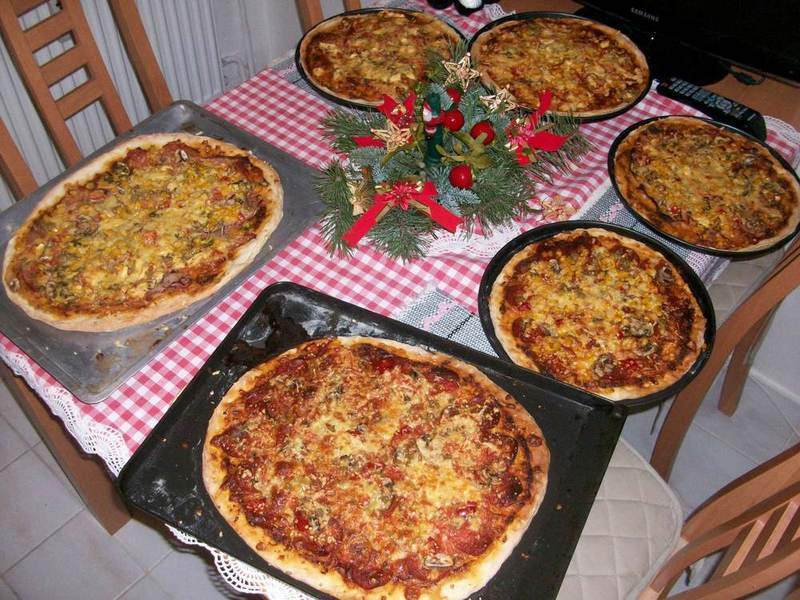
\includegraphics[height=4.5in]{dough_standard.JPG}
		\caption{\label{pic:dough_standard} Pizzas from the Standard dough, alternative baking}
	\end{figure}
	
	\begin{bclogo}[couleur = orange!30, logo = \bcsoleil]{\textbf{Dough Americana (for 7 medium pizzas)}}
		This should be strong enough dough for tossing and hand stretching in the air, with similar qualities like the Standard one, maybe just a bit more crunchy and crispy. \\
	
		Put the following into the bowl (respecting the order) in which you will mix the dough:
		\begin{itemize}
			\item 500ml of cold \textbf{water}
			\item 2l of dry \textbf{yeast}
			\item 4l of \textbf{salt}
		\end{itemize}
		Mix thoroughly and then add:
		\begin{itemize}
			\item 1kg of polohrub� (high gluten) \textbf{flour}
		\end{itemize}
		\hspace*{\fill}	
		
		\textbf{Mixing}: mix for about \textbf{25 minutes} (mix 5 minutes, rest 5 minutes, mix 15 minutes).
		\textbf{Preferable baking}: \textit{brick oven} - $280\,^{\circ}\mathrm{C}$ - \textit{6-8 minutes} \\
		\textbf{Alternative baking}: \textit{electric oven (bake from bottom)} - $240\,^{\circ}\mathrm{C}$ - \textit{12-14 minutes}
	\end{bclogo}
	\hspace{\fill}	
	
	\begin{figure}[h!]
		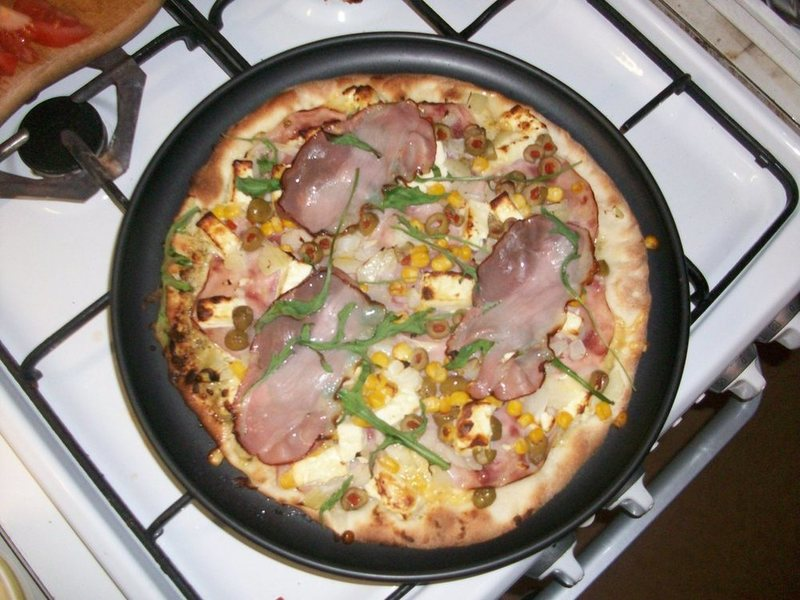
\includegraphics[height=4.5in]{dough_americana.JPG}
		\caption{\label{pic:dough_americana} A pizza from Americana dough, alternative baking}
	\end{figure}
	
	\begin{bclogo}[couleur = orange!30, logo = \bcsoleil]{\textbf{Neapolitan dough (for 7 medium pizzas)}}
		The Neapolitan dough should be thicker but softer and have a puffy but crispy crust. During the mixing process, it will be more sticky and generally, it is a weaker dough, thus pay attention when stretching it to avoid tearing/ripping of the dough. \\ 	
	
		Put the following into the bowl (respecting the order) in which you will mix the dough:
		\begin{itemize}
			\item 600ml of \textbf{water} ($18\,^{\circ}\mathrm{C}$) \footnote{This amount should be appropriate for \textit{hladk�} flour, in the original recipe using \textit{all-purpose} flour there was 725ml of water used. Clearly those two types of flour are not completely equivalent}
			\item 1.5l of dry \textbf{yeast}
			\item 2.75l of \textbf{salt}
		\end{itemize}
		Mix thoroughly and then continually add/mix in:
		\begin{itemize}
			\item 1kg of hladk� (all-purpose) \textbf{flour}
		\end{itemize}
		\hspace*{\fill}
		
		\textbf{Mixing}: mix for \textbf{4 minutes}. Let the dough rest for 5 minutes, then mix for additional 3-4 minutes. The dough should clear the sides of the bowl and stick a little to the bottom of the bowl. \\
		\textbf{Fermentation}: leave ferment in a fridge for at least 10 hours. \\
		\textbf{Stretching}: let the dough balls rest at room temperatures 2 hours before stretching, topping and baking them. Also, shape the disks a little bit thicker then e.g. those from Americana dough, the Neapolitan dough is weak and should not be made too thin. \\
		\textbf{Preferable baking}: \textit{wood-fired ovens} - $600\,^{\circ}\mathrm{C}$ - \textit{about 3 minutes} \\
		\textbf{Alternative baking}: \textit{electric oven (bake from bottom + whirling mode)} - $240\,^{\circ}\mathrm{C}$ - \textit{11-13 minutes}
	\end{bclogo}
	\hspace{\fill}
	
	\begin{figure}[h!]
		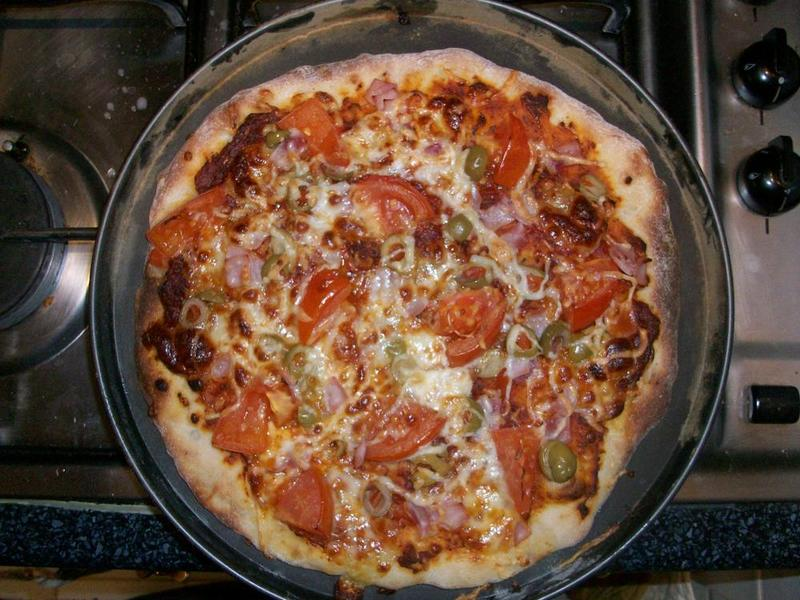
\includegraphics[height=4.5in]{dough_naples.JPG}
		\caption{\label{pic:dough_naples} A pizza from Neapolitan dough, alternative baking}
	\end{figure}
	
	\begin{bclogo}[couleur = orange!30, logo = \bcsoleil]{\textbf{Dough Danube Wednesday (for 7 medium pizzas)}}
		A pizza from this dough is very firm, crispy and crunchy. Rather then bending, the pizza will snap. On the contrary, the dough is rather weak, so stretch it on the table to prevent tearing and ripping. \\
	
		In a bowl, where you'll be mixing the dough, combine:	
		\begin{itemize}
			\item 1kg of hrub� \textbf{flour}
			\item 20g (3.5l) of \textbf{salt}
		\end{itemize}
		In another bowl, put:
		\begin{itemize}
			\item 575ml of \textbf{water} ($23\,^{\circ}\mathrm{C}$)
			\item 7g of fresh \textbf{yeast}
		\end{itemize}
		Let the yeast dissolve in the water. \\
		
		\textbf{Mixing}: continually pour in in the water/yeast mixture to the bowl with the flour, mix all the time. When combined, mix for about 10 more minutes. The dough should clear the sides of the bowl and stick a little to the bottom of the bowl. \\
		\textbf{Preferable baking}: \textit{wood-fired ovens} - $600\,^{\circ}\mathrm{C}$ - \textit{about 3 minutes} \\
		\textbf{Alternative baking}: \textit{electric oven (bake from bottom + whirling mode)} - $240\,^{\circ}\mathrm{C}$ - \textit{11-13 minutes}
	\end{bclogo}
	\hspace{\fill}
	
	\begin{figure}[h!]
		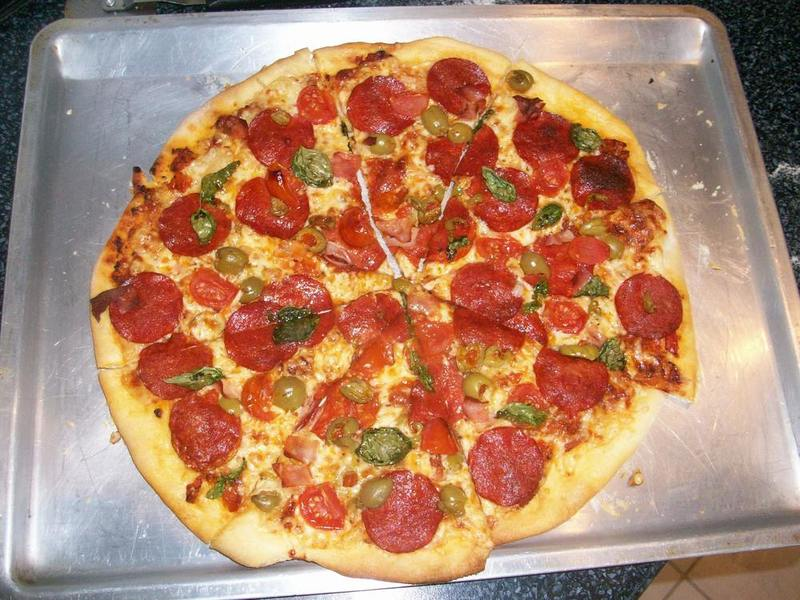
\includegraphics[height=4.5in]{dough_danube.JPG}
		\caption{\label{pic:dough_danube} A pizza from Danube Wednesday dough, alternative baking}
	\end{figure}
	
	\subsection{Dough mixing}
	
		Some general advices during \textbf{mixing of the dough}:
		\begin{itemize}
			\item The dough might be too sticky (in which case add more flour) or too dry and tearing apart (more water), but overall no big adjustments should be necessary.
			\item The texture should be smooth and the dough should not rip. 
		\end{itemize}
		\hspace*{\fill}
	
	\subsection{Dough ball shaping}
	
		After finishing the mixing, make \textbf{balls of dough} (about 220g for a medium and 350g for a large pizza). If the dough sticks to your hands, cover them with a little bit of olive oil. The shaping of the dough balls is explained e.g. here: \url{http://www.youtube.com/watch?v=_-8xEpX47Yc&t=3m57s}. \\
		
		Each shaped ball should be then covered in a thin layer of olive oil (to prevent drying of the dough) and put in a \textbf{dough-box} (picture \ref{pic:doughbox}), the bottom of which should also be covered with little olive oil. The box should then be hermetically closed, again to prevent drying of the dough by the air. \\
		
		Leave in a fridge to \textbf{ferment} for at least 4 hours, but preferably longer (overnight). \\
		
		\begin{figure}[h!]
			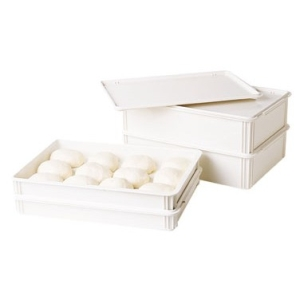
\includegraphics[height=3in]{dough-box.jpeg}
			\caption{\label{pic:doughbox} Dough-box}
		\end{figure}
		
	\subsection{Stretching of the dough}

		As for \textbf{stretching the dough}, I recommend seeing the following videos:
		\begin{enumerate}
			\item \url{http://www.youtube.com/watch?v=GuOzvmQkZgs} - stretching of the dough, explained
			\item \url{https://www.youtube.com/watch?v=35MZN4vXfz8&list=UUI-Iz-mKmsy30s4io8wkq7w&index=11} - one of the world's best pizza makers explaining how to flip the dough
			\item \url{http://www.youtube.com/watch?v=SBdpyfeUobM&t=3m53s} - a world record in making 3 pizzas
		\end{enumerate}
		\hspace*{\fill}
		
		However, the stretching technique differs with the dough used. With strong dough one can toss, spin and stretch the dough in the air without problems (video 2). With softer and weaker doughs it is better to stretch the dough on a smooth (e.g. marble, stainless steel) surface (video 1). The factors that make the dough stronger are (among others):
		\begin{itemize}
			\item \textbf{amount of gluten/protein} in the flour - high-gluten flour based dough would be more suitable for tossing then one made from all-purpose flour
			\item \textbf{water temperature} - the colder, the stronger the dough
			\item \textbf{amount of water} - too much water means stickier and weaker dough
			\item \textbf{amount of salt} - more salt means stronger dough
			\item see \url{https://www.youtube.com/watch?v=HilN-bajNqQ}
		\end{itemize}
		\hspace*{\fill}
		
		Once the dough is stretched, top it and put to the oven without much further delays. 
		
		%TODO - why? Do not leave the shaped disk of pizza dough (topped or un-topped) 
	
	\subsection{Baking}
	
		Finally, a few words about the \textbf{baking}. Most of you reading this probably do not have an access to an original brick ovens or wood-fired ovens that could be found in most pizzerias (neither do I). However, even with an ordinary electric or gas oven, one can achieve pretty decent results. \\
		
		Most ovens are able to bake from the bottom (sometimes only from the bottom) and can achieve temperatures of about $250\,^{\circ}\mathrm{C}$. While this is not ideal for most of the pizzas (depends largely on the type of the dough), it should be sufficient to get a pretty good pizza in almost any case. \\
		
		Some ovens have an air-whirling mode which somehow makes it possible to bake several pizzas at the same time. However, be careful to have the bottom baked sufficiently, as this is often not the case with baking at the air-whirling mode. \\
		
		Usually, you just have to \textbf{experiment}. Always measure the time it took you to make the pizza and notice the following:
		\begin{itemize}
			\item Is the bottom baked properly? This is the most important criterion. The bottom is baked sufficiently if there are the first hints of black (burned) spots on it (but just \textit{first hints}).
			\item Are the edges (crust) brown (caramelized) enough? Again, they should be brown with the first hints of black spots. For well baked crust, see pictures of pizza in this paper.
		\end{itemize}
		\hspace*{\fill}
		
		Depending on which part gets baked too quickly, you can try:
		\begin{itemize}
			\item Move the pizzas vertically in the oven (closer or farther away from the source of the heat)
			\item Turn on air-whirling mode in addition to "baking-from-bottom" if bottom is done too quickly
		\end{itemize}
		\hspace*{\fill}
		
		Also, if you bake on pizza plates, butter them and sprinkle with flour to prevent stickiness, or use pizza plates with little holes in them. \\
		
		Pizzas usually taste the best straight out of the oven - so try make sure to get the timing correctly to serve the pizzas freshly baked.
		
\section{Sauce}	
	
	\begin{bclogo}[couleur = red!30, logo = \bcpoisson]{\textbf{Sauce Standard (for 4 medium pizzas)}}
		You need:
		\begin{itemize}
			\item 2 medium size \textbf{tomatoes}
			\item 70g of \textbf{tomato paste}
			\item 4 crushed \textbf{garlics}
			\item 0.5l of \textbf{salt}
			\item 0.5l of \textbf{black pepper}
			\item 10g of crushed \textbf{oregano}
			\item 1L of crushed \textbf{basil leaves}
			\item 2L of \textbf{water}
			\item 3l of \textbf{olive oil}
		\end{itemize}
		\hspace*{\fill}
		
		Crush the tomatoes, add everything else and mix thoroughly.
	\end{bclogo}
	\hspace{\fill}
	
	\begin{bclogo}[couleur = red!30, logo = \bcpoisson]{\textbf{White sauce (for 4 medium pizzas)}}
		You need:
		\begin{itemize}
			\item 4L of \textbf{olive oil}
			\item 1 small \textbf{onion}, chopped to little pieces
			\item 4 crushed \textbf{garlics}
			\item 200g of heavy cream (40\% fat whipped cream in liquid state)
			\item 0.5l of \textbf{salt}
			\item 0.5l of \textbf{black pepper}
			\item 5g of crushed \textbf{marjoram/thyme} (1.5L)
		\end{itemize}
		\hspace*{\fill}		
		
		Saut� the onion for 5-6 minutes on the olive oil over medium heat. Add garlic and stir for 1 minute. Pour in the cream, lower the heat a bit and cook for 3 more minutes - the cream should thicken a bit. \\
		
		Remove from heat and season with salt, pepper and marjoram/thyme. Let cool completely before using.
	\end{bclogo}
	\hspace{\fill}
	
	\begin{bclogo}[couleur = red!30, logo = \bcpoisson]{\textbf{Bistro white sauce (for 4 medium pizzas)}}
		You need:
		\begin{itemize}
			\item 6L of \textbf{olive oil}
			\item 5 crushed \textbf{garlics}
			\item 9g of crushed \textbf{oregano} (3L)
		\end{itemize}
		\hspace*{\fill}		
		
		Mix everything together.
	\end{bclogo}
	\hspace{\fill}
	
	\pagebreak	
	
	\section{Toppings}
	
	\begin{bclogo}[couleur = blue!30, logo = \bctrefle]{\textbf{Mediterranean (1 medium pizza)}}
		Top the pizza with following, respecting the order:
		\begin{itemize}
			\item Grated \textbf{Mozzarella} and \textbf{Eidam} (mixed in ratio 1/2)
			\item \textbf{Onions} rings
			\item \textbf{Ham} cut to squares 1x1 cm
			\item \textbf{Olives} cut to thirds of their sizes
			\item \textbf{Tomatoes} cut to small cubes (0.5 cm)
			\item \textbf{Feta cheese} cut to small cubes, like tomatoes
		\end{itemize}
	\end{bclogo}
	\hspace{\fill}
	
	\begin{bclogo}[couleur = blue!30, logo = \bctrefle]{\textbf{Ham \& mushroom (1 medium pizza)}}
		Top the pizza with following, respecting the order:
		\begin{itemize}
			\item Grated \textbf{Mozzarella} and \textbf{Eidam} (mixed in ratio 1/2)
			\item \textbf{Ham} cut to squares 1x1 cm
			\item \textbf{Champignons} (sliced)
			\item \textbf{Tomatoes} cut to small cubes (0.5 cm)
			\item \textbf{Olives} cut to thirds of their sizes
		\end{itemize}
	\end{bclogo}
	\hspace{\fill}
	
	\begin{figure}[h!]
		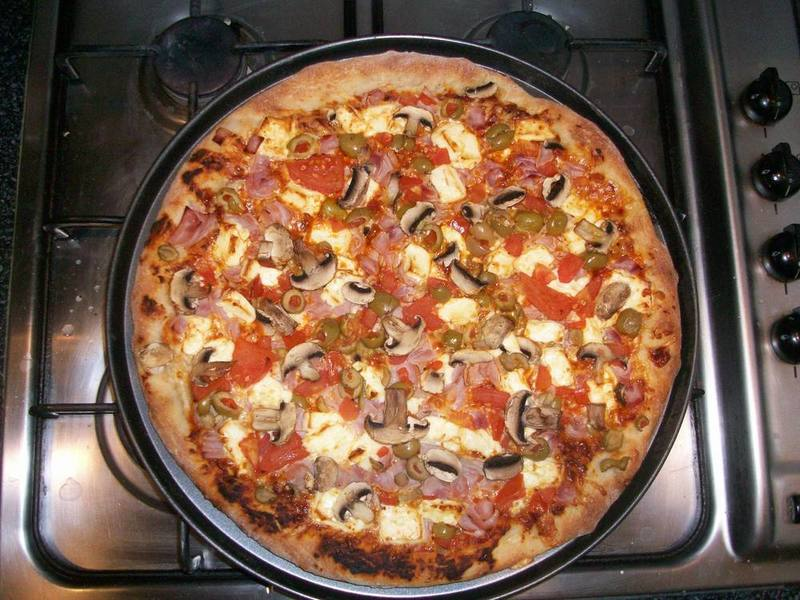
\includegraphics[height=4.5in]{toppings_hammush.JPG}
		\caption{\label{pic:toppings_hammush} Ham \& mushroom pizza (with some added Feta cheese)}
	\end{figure}
	
	\pagebreak
	
	\begin{bclogo}[couleur = blue!30, logo = \bctrefle]{\textbf{Pepperoni (1 medium pizza)}}
		Top the pizza with following, respecting the order:
		\begin{itemize}
			\item Grated \textbf{Mozzarella} and \textbf{Eidam} (mixed in ratio 1/2)
			\item \textbf{Pepperoni} (��ip�k)
			\item \textbf{Olives} cut to thirds of their sizes
			\item Optionally \textbf{hot peppers} (fefer�ny, jalapenos)
		\end{itemize}
	\end{bclogo}
	\hspace{\fill}
	
	\begin{figure}[h!]
		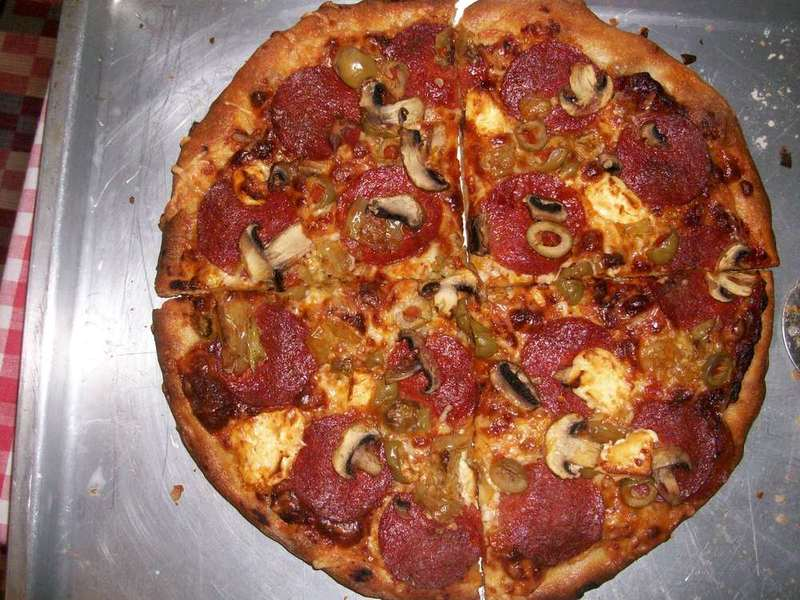
\includegraphics[height=4.5in]{toppings_pepperoni.JPG}
		\caption{\label{pic:toppings_pepperoni} A bit adjusted pepperoni pizza}
	\end{figure}
	
	\pagebreak
	
	\begin{bclogo}[couleur = blue!30, logo = \bctrefle]{\textbf{BBQ chicken (1 medium pizza)}}
		Top the pizza with following, respecting the order:
		\begin{itemize}
			\item Grated \textbf{Mozzarella} and \textbf{Eidam} (mixed in ratio 1/2)
			\item \textbf{Grilled chicken} cut to small cubes
			\item \textbf{Onion} rings
			\item \textbf{BBQ sauce}
			\item \textbf{Sweet peppers} (baranie rohy)
		\end{itemize}
	\end{bclogo}
	\hspace{\fill}
	
	\begin{figure}[h!]
		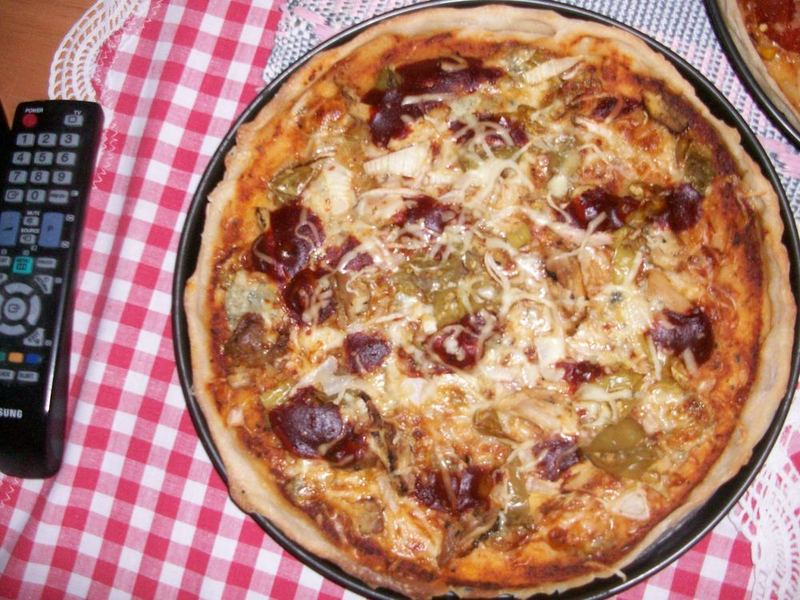
\includegraphics[height=4.5in]{toppings_bbq.JPG}
		\caption{\label{pic:toppings_bbq} BBQ chicken pizza}
	\end{figure}
	
	\pagebreak
	
	\begin{bclogo}[couleur = blue!30, logo = \bctrefle]{\textbf{Prosciutto (1 medium pizza)}}
		Top the pizza with following, respecting the order:
		\begin{itemize}
			\item Pieces of \textbf{Mozzarella Bocconcini}
			\item Pieces of \textbf{tomatoes}
			\item \textbf{Fresh basil leaves}
			\item Sprinkle with \textbf{Parmesan} cheese
		\end{itemize}
		Right after taking out of the oven add:
		\begin{itemize}
			\item \textbf{Prosciutto}
		\end{itemize}
	\end{bclogo}
	\hspace{\fill}
	
	\begin{figure}[h!]
		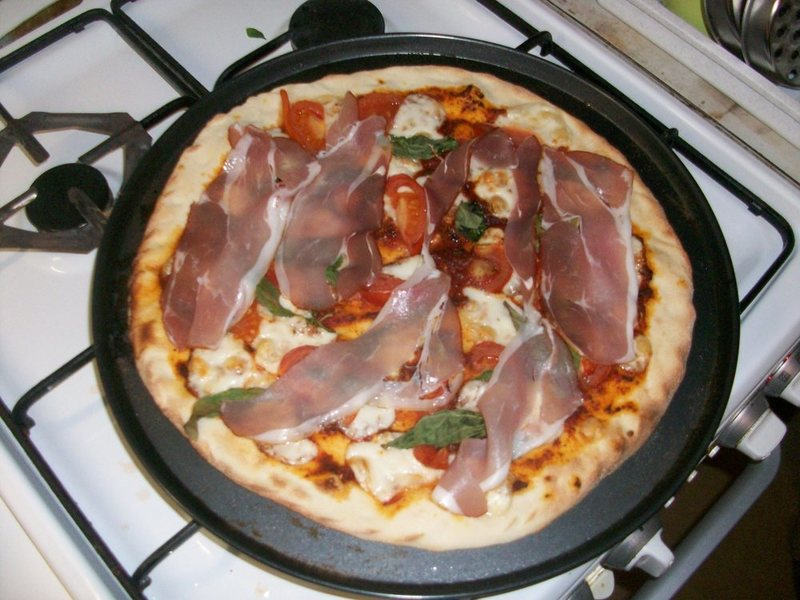
\includegraphics[height=4.5in]{toppings_prosciutto.JPG}
		\caption{\label{pic:toppings_prosciutto} Prosciutto pizza (without Parmesan cheese)}
	\end{figure}
	
	\pagebreak
	
	\begin{bclogo}[couleur = blue!30, logo = \bctrefle]{\textbf{Bryndza pizza (1 medium pizza)}}
		Top the pizza with following, respecting the order:
		\begin{itemize}
			\item Little pieces of \textbf{Bryndza}
			\item \textbf{Pepperoni} or sausage (klob�sa)
			\item \textbf{Onion}
			\item Just a little of \textbf{ham} (cut to smaller pieces)
		\end{itemize}
		\hspace*{\fill}
		
		I would suggest to use Bistro white sauce for this pizza, though you may experiment with other sauces as well.
	\end{bclogo}
	\hspace{\fill}
	
	\begin{figure}[h!]
		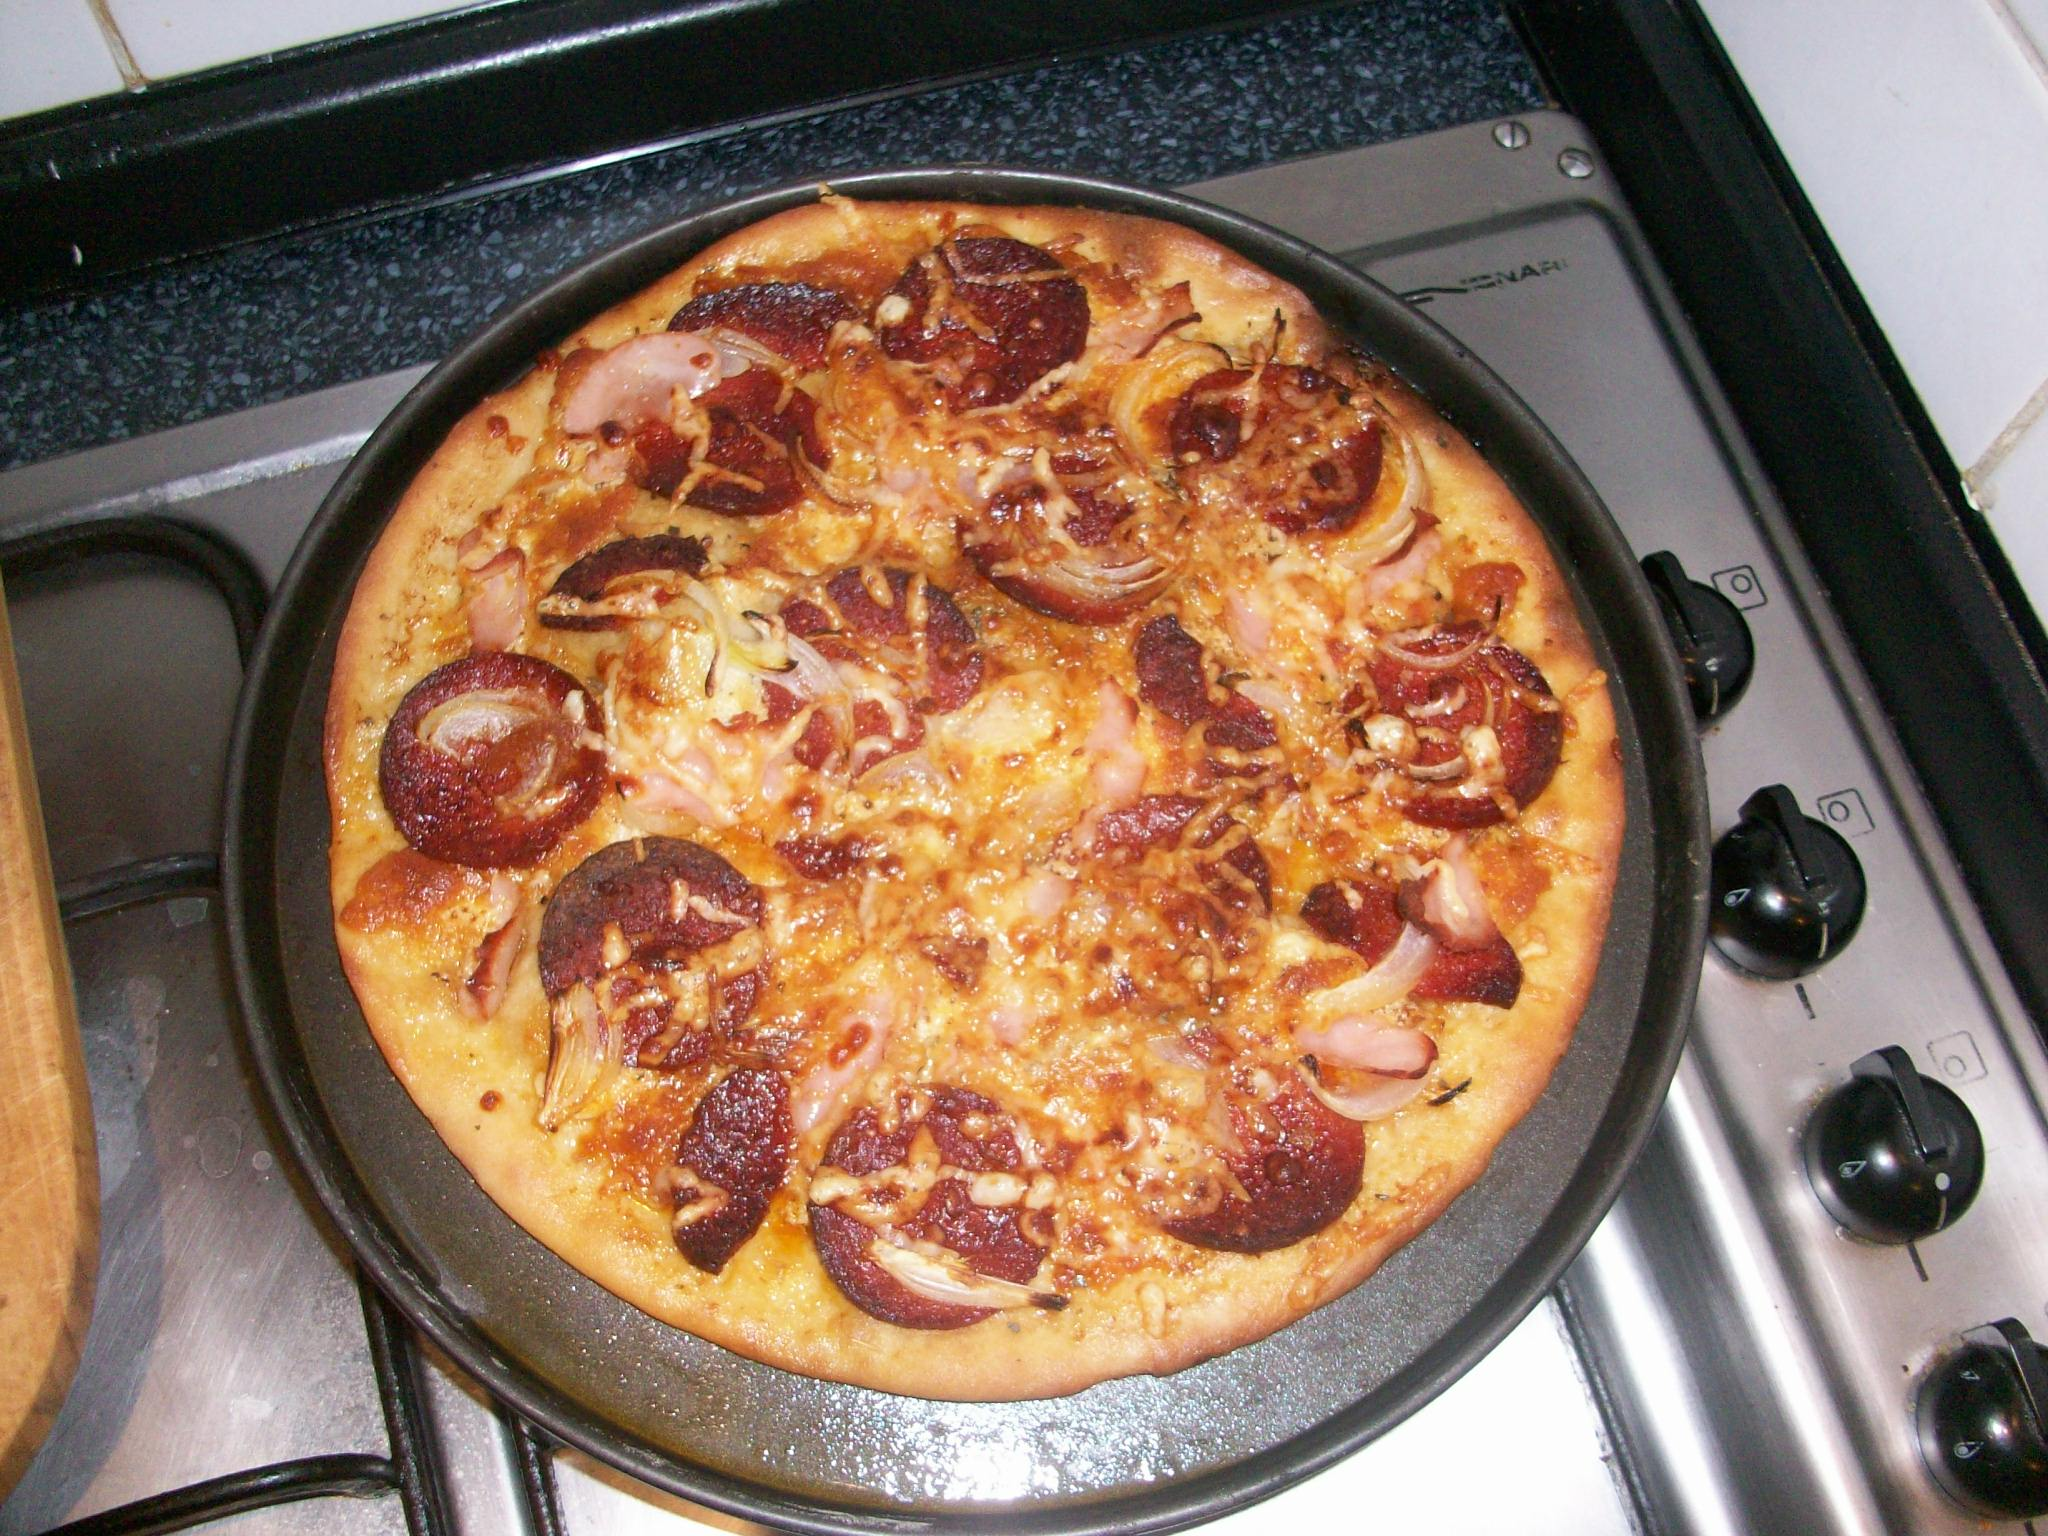
\includegraphics[height=4.5in]{toppings_bryndza.JPG}
		\caption{\label{pic:toppings_bryndza} Bryndza pizza, with a little sprinkled cheese on top}
	\end{figure}
	
	Some \textbf{general advices}:
	\begin{itemize}
		\item If you feel the pizza would be too dry, sprinkle the top with some olive oil. However you can do that even if the pizza should not be too dry
		\item Some people like to see the cheese also on the top - in that case, sprinkle the top with a little more cheese
	\end{itemize}
	
	\section{The pizzas}	
	
	You can now make your own pizza from the three basic building blocks - the dough, sauce and the toppings. \\
	
	Some good combinations I like:
	\begin{itemize}
		\item Naples - Standard - Prosciutto
		\item Danube Wednesday - White - Pepperoni
		\item Americana - White - Mediterranean		
	\end{itemize}
	
	\section{Outro}
	There are plenty of recipes or pizza-dedicated websites on the internet or even as books. My favourites are the following:
	\begin{itemize}
		\item Peter Reinhart's book - \textbf{American Pie: My Search for the Perfect Pizza}~\cite{reinhart03}. Maybe the most famous publication there is to be found concerning pizza-making. 
		\item Billy Reisinger's website - \textbf{The Amateur Guide to Making Pizza}~\cite{reisinger}
		\begin{itemize}
			\item \url{http://billyreisinger.com/pizza_walkthrough.html} 
		\end{itemize}
		\item \textbf{Pizza therapy website}~\cite{Therapy} 
		\begin{itemize}
			\item \url{http://pizzatherapy.com/}
		\end{itemize}
	\end{itemize}
	
	
	
	
	
	
	
	
	
	
	
	
	
	
	
	
	
	
	
	
	
	
	
	
	
	
	%---------------------------------------------------------------------
    %   SVK
    %---------------------------------------------------------------------
	\else
	
	\section{�vod}
	Basically, all pizzas consist of 4 parts of which some might be left out:
	\begin{enumerate}
		\item \textbf{dough}
		\item \textbf{sauce}
		\item \textbf{cheese}
		\item \textbf{toppings}
	\end{enumerate}
	\hspace{\fill}
	
	I put them on the pizzas in the mentioned order, though sometimes some of the cheese is put under the toppings (depends what do you want to have more thoroughly baked).
	
	\section{Dough}
		\begin{bclogo}[couleur = yellow!30]{\textbf{Dough (for 8 medium pizzas)}}
			Put the following into the bowl (respecting the order) where you will mix the dough:
			\begin{itemize}
				\item 500ml of \textbf{water} (slightly, but only slightly warm!)
				\item \textbf{yeast}, 2.5 x 2.5 x 2.5 cm cube. Alternatively 1 sachet of dry yeast
				\item 4l of \textbf{salt}
				\item 1l of \textbf{sugar}
				\item 1L of \textbf{olive oil}
			\end{itemize}
			Mix thoroughly and then add:
			\begin{itemize}
				\item 1kg of all-purpose (polohrub�) \textbf{flour}
			\end{itemize}
			\hspace{\fill}
		\end{bclogo}
		
		The dough should be mixed for about \textbf{25 minutes}. It might be too sticky (in which case add more flour) or too dry and tearing apart (more water), but overall no big adjustments should be necessary. \\
		
		After finishing the mixing, make balls of dough (about 200g for medium and 330g for large pizza). The shaping of the dough balls if explained e.g. here: \url{http://www.youtube.com/watch?v=_-8xEpX47Yc&t=3m57s}. Cover each shaped ball in a thin layer of olive oil (to prevent drying of the dough) and put in a dough-box (picture \ref{pic:doughbox}) with bottom also covered with little olive oil. The box must then be closed (hermetically), again to prevent drying of the dough by air. Leave in a fridge to ferment for at least 4 hours.
	
	\begin{figure}[h!]
		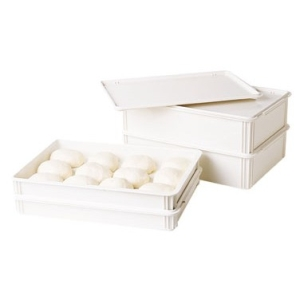
\includegraphics[height=1.65in]{dough-box.jpeg}
		\caption{\label{pic:doughbox} Dough-box}
	\end{figure}

		As for stretching the dough, I recommend seeing the following videos:
		\begin{itemize}
			\item \url{http://www.youtube.com/watch?v=GuOzvmQkZgs} - stretching of the dough, explained
			\item \url{http://www.youtube.com/watch?v=SBdpyfeUobM&t=3m53s} - a world record in making 3 pizzas
		\end{itemize}
	
	\section{Sauce}	
	Taka ta klasicka co robim je: 200g pretlaku, rozdrvene 4 cesnaky, 1/2l sol, 1/2l korenie, sacok drveneho oregana (10g), nadrvene basil leaves (1l), asi 1/3deci vody, olivovy olej (tak 3 lyzicky) - vsetko rozmixovat a premiesat.
	
	\section{Cheese}	
	Davam mix mozzarella a eidam (v USA davali white cheddar). Staci 200g mozzarelly a 400g eidamu.
	
	\section{Toppings}
	Moje oblubene kombinacie:
	\begin{itemize}
		\item mediterranean: sunka, olivy, sampinony, paradajky, feta syr, cibula
		\item pepperoni: scipak, feferony, olivy, baranie rohy (resp. sweet peppers)
		\item bbq chicken: grilovane kuracie prsia, cibula, bbq omacka, baranie rohy (resp. sweet peppers)
		\item ham \& mushroom: sunka, sampinony, paradajky, olivy
	\end{itemize}

	\section{Baking}
	Kedze nemam pizza stone, peciem na plechoch (pomastene herou a pomucene). Rura je v mode kde viri horuci vzduch, teda nepecie len z jednej strany. A teplota na maxime (u mna 240c, v USA bola 560f = cca 290c). Takto su hotove za cca 20 minut. 
	
	\section{The pizzas}
	
	\section{Outro}
	Cely postup krok-za-krokom aj s obrazkami je inac dobre spraveny tu \url{http://billyreisinger.com/pizza_walkthrough.html} .	
	
	\fi

    %---------------------------------------------------------------------
    %   bibliography
    %---------------------------------------------------------------------
    \bibliographystyle{is-alpha}
    %compile latex, bibtex, latex, latex
    \bibliography{bibl}{}
\end{document}
